\section{Aufbau}
    Im Folgenden wird der Aufbau des Algorithmus näher beschrieben. 
    Nach einem kurzem Überblick werden die einzelnen Subsysteme detailliert erklärt.
    \subsection{Grundlegende Struktur}
    % oberflächliche Beschreibung des systems

    Es soll eine Liste an Layern, anhand der zuvor definierten Ziele, generiert werden.
    Die oberflächliche Struktur, des Generators, ist im unteren Flussdiagramm dargestellt.
    Für eine gegebene Anzahl an Layern in einer Rota wird für jedes Layer folgende Routine ausgeführt:

    \begin{itemize}
        \item wähle einen Modus, gewichtet nach den Mode-Wahrscheinlichkeiten $w_g$ und dem Mode-Spacing $\Delta_g$
        \item für den gewählten Modus werden die validen Maps gefiltert
        \begin{itemize}
            \item zunächst wird geprüft, welche Map im Modus repräsentiert ist
            \item aus den vorhanden Maps wird nach dem Distanz-Vote-Weight $w_m$ gewichtet eine Map gezogen
        \end{itemize}
        \item für die gezogene Map wird gewichtet nach dem Layerweight $w_l$ ein Layer gezogen
        \item die gezogenen Maps verbleiben für eine feste Maplänge im Memory-Kernel und sind damit für die nächsten Map Ziehungen nicht verfügbar
    \end{itemize}
    Im Folgenden werden die drei verschiedenen Schritte genauer erklärt und die verwendeten Weights definiert. 
    \begin{figure}[htbp]
        \centering
        \includegraphics[width=0.8\textwidth]{FlowChartSuperficial.png}
        \caption{Oberflächlicher Ablauf des Generators.}
    \end{figure}

    \subsection{Aufbau im Detail - Mode}
        Wie zuvor erwähnt gibt es zwei Faktoren, welche die Ziehung des Modus beeinflussen:
        \begin{itemize}
            \item [1.] die Modeweights die zuvor gesetzt wurden $w_g$ 
            \item [2.] das Modespacing $\Delta_g$
        \end{itemize}
        Des Weiteren erlaubt der Generator eine Gruppierung der Modes in sogenannte ''Pools''. 
        Es gibt immer einen sogenannten \textit{main}-Pool. 
        Ohne weitere Einstellungen ist jeder Modus, der gespielt werden soll, automatisch im Main-Pool enthalten. 
        Neben diesem können noch weitere Pools definiert werden. 
        In der momentanen Fassung existieren drei Pools:
        \begin{itemize}
            \item \textbf{main}: Der zuvor erwähnte Standard-Pool, beinhaltet \textit{RAAS} und \textit{AAS}
            \item \textbf{intermediates}: Beinhaltet die Modi \textit{Invasion} und \textit{TC}
            \item \textbf{reste}: Beinhaltet \textit{Destruction} und \textit{Insurgency}
        \end{itemize}

        Das \textbf{Modespacing} $\Delta_g\in{0,...,N}$ ist eine Zahl größer $0$ und maximal die Anzahl der Layer in einer Rota.
        Es sorgt nun dafür, dass für eine gegebene Anzahl an Runden nur der Main-Pool gezogen werden darf, wodurch eine \glqq{}Mindestzeit\grqq{} zwischen z.b. zwei Invasion Layern garantiert wird.
        Sollte die Zeitspanne seit dem letzten nicht-main Modus größer sein als das Modespacing, so wird mit den Pool und Mode-weights gewichtet ein Gamemode gewählt. 
        Hierbei wird erst der Pool ausgewählt und anschließend im Pool der Modus. 
        Es ist zu beachten, dass dies dazu führen kann und wird, dass nicht direkt nach Ablauf des Modespacings ein andere Pool drankommen muss. 
        Das Design wurde mit Absicht so gewählt, um repetitive Modes zu verhindern.

        Das Modeweight $w_g$ setzt sich damit zusammen aus der Wahrscheinlichkeit den enthaltenen Pool zu ziehen und den Modus 
        \begin{equation}
            w_g = \mathbb{P}(G=g|P=p) = \mathbb{P}(G=g)\mathbb{P}(P=p)
        \end{equation}
        wobei hier $G$ und $P$ die Zufallsvariablen ''Gamemode'' und ''Pool'' darstellen sollen.
        Durch das Modespacing ist die Wahrscheinlichkeit einen Modus zu ziehen gegeben durch 
        \begin{equation}
            \mathbb{P}(G=g) = \frac{1}{N}\sum_{j=0}^{k_0}j\binom{N-j \Delta_g}{j}w_g^j(1-w_g)^{N-j(\Delta_g+1)}
        \end{equation}
        mit $w_g$ das oben definierte Weight, $N$ die Anzahl gezogener Layer und $k_0=\lfloor\frac{N}{N_0}\rfloor$ die maximale Anzahl an Zügen des Modus.
        Der interessierte Leser vermag eine Herleitung im Anhang zu finden.

        Anschließend wird geprüft ob die Verfügbaren Maps den gewählten Modus enthalten. Sollte dies nicht der Fall sein so wird der Modus in einem Buffer gespeichert und es wird erneute ein Modus zufällig gewählt. 
        Der Buffer wird bei der nächsten Gelgenheit abgearbeitet.
    \subsection{Aufbau im Detail - Map}
        Das Weight errechnet sich als Produkt aus einem ''Distanz-Weight'' und einem ''Mapvote-Weight''. 
        \begin{equation}
            w_m(m,d,v) = \frac{1}{\mathcal{N}}w_d(d,m)w_v(v,m)
        \end{equation}
        wobei $\mathcal{N}$ das Produkt-Weight normiert sodass $\sum_m w_m = 1$.
        \subsubsection{Distanzweight}
            Das Distanzweight ist eine allgemeine stückweise stetige Funktion definiert durch
            \begin{equation}
                w_d : \mathbb{R}^+ \rightarrow \mathbb{R}^+, d \mapsto w_d(d),
            \end{equation}
            und der Nebenbedingung $w_d(d)\overset{d\rightarrow 0}{\longrightarrow}0$.
            In der momentanen Version ist die Funktion gegeben durch
            \begin{equation}
                w_d(d) = 1_{[0,d_\text{min}]}(d)
            \end{equation}
            mit $d_\text{min}\geq 0$ als Mindestdistanz. 
            Sollte eine Map näher als $d_\text{min}$ an einer zuvor gezogenen Map liegen ist das Distanzweight und damit das Mapweight $0$ und wird damit nicht gezogen. 
        \subsubsection{Mapvoteweight}
            Das Mapvoteweight wird aus dem Mapvote berechnet aus 
            \begin{equation}
                w_v(v) = \sum_{i,j = 0}^2 a_{ij}x^i y^j
            \end{equation}
            wobei $x$ die Anzahl an verbundenen Maps ist und $y$ die Mapwahrscheinlichkeit errechnet aus den Layervotes.
            Die Koeffizienten $a_{ij}\in\mathbb{R}$ müssen vorerst numerisch bestimmt werden.  
            wobei $v$ die Summe aller Layervotes eines Modus einer Maps ist und $a$ und $b$ zwei freie Parameter sind.
            Während $a$ die Steigung moduliert kann mit $b$ ein Offset erzeugt werden.
            Die Sigmoid funktion erlaubt es ein kontinuierliches weight zu definieren wodurch eine Map oder ein Layer nicht abrupt verschwindet sondern langsam ändert.
            \begin{figure}[htbp]
                \centering
                \includegraphics[width=0.85\textwidth]{plot_sigmoid.pdf}
                \caption{Die Sigmoidfunktion für mehrere Werte $a$ und $b$. 
                            Für $b=0$ ist für alle Werte $a$ $f(0)=1/2$.
                            Der Parameter $b$ dient als Offset.}
            \end{figure}
    Jeder Map die im Modus enthalten ist wird ein Mapvoteweight $w_m$ und ein Distanzweight $w_d$ zugeordnet. 
    Aus dem Produktweight wird anschließend die Map gezogen. 
    Hier kommt noch hinzu dass die Distanzweights vom Memory-Kernel abhängen. 
    In der momentanen Implementierung bedeutet dies, dass eine Map, welche in den letzten $k$ Runden gezogen wurde, nicht nochmal dran kommen kann. 
    Effektiv heißt dies $w_d=0$ für diese Map. 
    Für den seltenen Fall, dass keine Map für einen Modus verfügbar ist, weil alle in Frage kommenden Maps zurzeit gesperrt sind wird der Modus in den sogenannten \textbf{Mode-Buffer} verlegt. \todo{timbow schreib mal den satz um}
    Dieser wird beim Ziehen des nächsten Modus abgearbeitet. 
    Das bedeutet ein Modus wird \glqq{}ge-queued\grqq{} und kommt bei der nächst passenden Gelegenheit dran. 
    
    \subsection{Aufbau im Detail - Layer}
    Sobald eine Map ausgewählt wurde wird das Layer gewichtet nach dem Layerweights $w_l$ gezogen. 
    Diese hängen nur von den Mapvotes ab welche mit der vorher genannten Sigmoidfunktion moduliert werden.
    Damit ist dann für $N_l$ Layer einer Map 
    \begin{equation}
        w_l(j) = \frac{1}{\sum_{m=0}^{N_l}\frac{1}{\sum_{m=0}^{N_l}\left[1+\exp\left(-a(v_m+b)\right)\right]}}\frac{1}{1+\exp\left(-a(v_j+b)\right)}
    \end{equation} 
    mit $v_j$ die Mapvote-Zahl des Layers $j$ der gegebenen Map.
    \begin{figure}[htbp]
        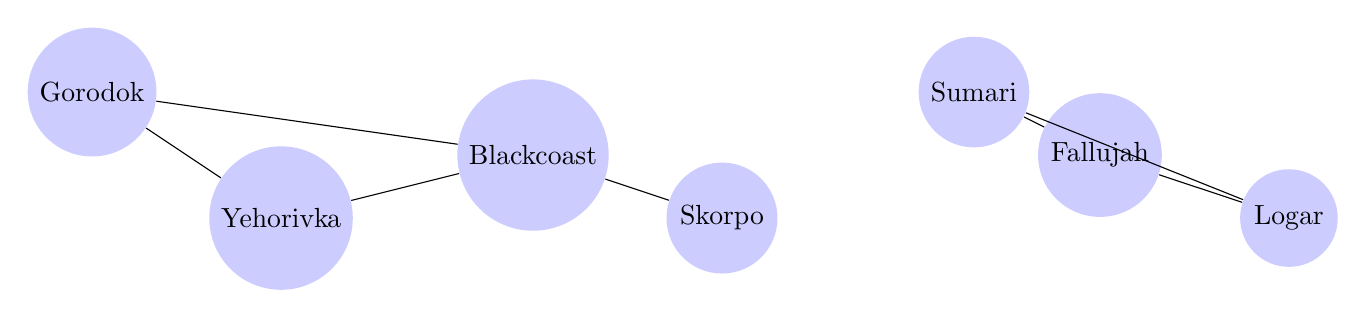
\begin{tikzpicture}
            [scale=.8,auto=left,every node/.style={circle,fill=blue!20}]
            \node (n1) at (1,10) {Gorodok};
            \node (n2) at (4,8)  {Yehorivka};
            \node (n3) at (8,9)  {Blackcoast};
            \node (n4) at (11,8) {Skorpo};
            \node (n5) at (15,10) {Sumari};
            \node (n6) at (20,8)  {Logar};
            \node (n7) at (17,9)  {Fallujah};
            \foreach \from/\to in {n1/n2,n1/n3,n2/n3,n3/n4,n5/n6,n5/n7,n6/n7}
            \draw (\from) -- (\to);  
        \end{tikzpicture}
    \caption{Cluster}
    \end{figure}
    \todo{cluster abbildung wurde nicht in den Text eingebunden, überflüssig ?}